\item Una barra homogénea de masa $m$ y largo $l$, puede moverse en un plano vertical a causa de un pivote ubicado en uno de sus extremos. La barra está sumergida en un fluido, el cual le ejerce una fuerza de fricción proporcional a la velocidad de su centro de masa, tal que $\vec{F}_{r}=-b\,\vec{v}_{\scriptsize{\text{CM}}}$, donde $b$ es la constante de amortiguamiento. Considere que el fluido solo ejerce la fuerza de roce sobre la barra.
	\begin{figure}[tbph]
		\centering
		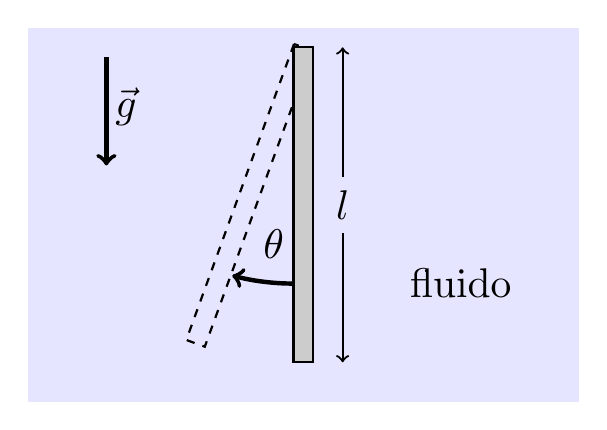
\begin{tikzpicture}
			%prob11.pdf
			\fill [fill=blue!10!white] (-3.5,.25)rectangle(3.5,-4.5);
			\draw [dashed,thick,rotate=-20] (-.125,0)rectangle(.125,-4);
			\filldraw [fill=black!20!white,thick] (-.125,0)rectangle(.125,-4);
			\draw [ultra thick,->] (-2.5,-.125)--(-2.5,-1.5);
			\draw [<->,thick] (.5,0)--(.5,-4);
			\draw [->,ultra thick] (-.125,-3)arc(270:255:3);
			\draw [dotted]
				(.5,-2) node[scale=1.5,fill=blue!10!white] {\(l\)}
				(-.375,-2.5) node[scale=1.5] {\(\theta\)}
				(-2.25,-.75) node[scale=1.5] {\(\vec{g}\)}
				(2,-3) node[scale=1.5] {fluido}
				;
		\end{tikzpicture}
	\end{figure}
	\begin{enumerate}[a)]
		\item Determine la ecuación de movimiento para el movimiento oscilatorio de la barra en torno a su posición de equilibrio, considerando pequeñas oscilaciones.
		
		\item Calcule el valor crítico de la constante de amortiguamiento, $b_{\text{c}}$, que impide que la barra oscile.
		
		\item Suponga que $b=b_{\text{c}}/2$. Obtenga el periodo para pequeñas oscilaciones.	
	\end{enumerate}

\underline{Soluci\'on:}

\begin{enumerate}[a)]
	\item \begin{figure}[tbph]
		\centering
		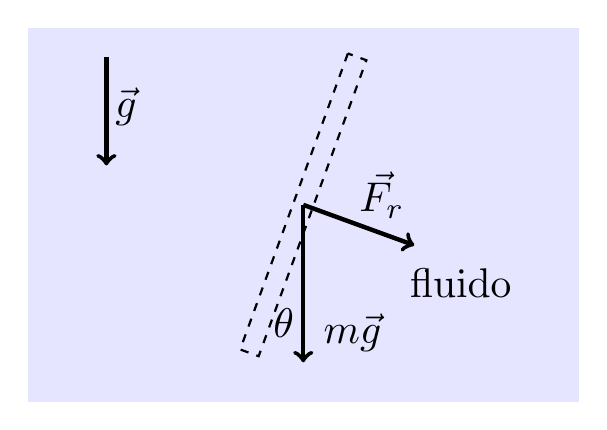
\begin{tikzpicture}
		%prob11.pdf
		\fill [fill=blue!10!white] (-3.5,.25)rectangle(3.5,-4.5);
		\begin{scope}[shift={(0,-2)},rotate=-20]
		\draw [dashed,thick] (-.125,2)rectangle(.125,-2);
		\draw [->, ultra thick,rotate=20] (0,0)--(0,-2);
		\draw [->, ultra thick] (0,0)--(1.5,0);		
		\end{scope}
		\draw [ultra thick,->] (-2.5,-.125)--(-2.5,-1.5);
		\draw [dotted]
		(1,-1.875) node[scale=1.5] {\(\vec{F_r}\)}
		(-.25,-3.5) node[scale=1.5] {\(\theta\)}
		(.625,-3.625) node[scale=1.5] {\(m\vec{g}\)}
		(-2.25,-.75) node[scale=1.5] {\(\vec{g}\)}
		(2,-3) node[scale=1.5] {fluido}
		;
		\end{tikzpicture}
	\end{figure}
	
	De acuerdo al diagrama de cuerpo libre de la figura, en donde se representan las \'unicas dos fuerzas que realizan torque respecto del pivote, podemos escribir
	\begin{equation*}
		I \ddot{\theta} = -\frac{l}{2}b\frac{l}{2} \dot{\theta} -mg\frac{l}{2} \sin \theta\,,
	\end{equation*}
	donde hemos usado que $v_{\scriptsize{\text{CM}}}=(l/2) \dot{\theta}$. Como el momento de inercia de la barra respecto al pivote es $I=(1/3)ml^{2}$, para peque\~nas oscilaciones ($\sin \theta \approx \theta$) la ecuación de movimiento viene dada por
	\begin{equation*}\label{ecmovfinal}
		\ddot{\theta} + \frac{3b}{4m} \dot{\theta} + \frac{3g}{2l}\theta=0\,.
	\end{equation*}

	\item Escribiendo la ecuación de movimiento en la forma 
	\begin{equation*}\label{ecmovgeneral}
		\ddot{\theta} + 2\gamma \dot{\theta} + \omega_{0}^{2}\,\theta=0\,,
	\end{equation*}
	para los casos en que $\gamma^2-\omega_{0}^{2}\leq 0$, la soluci\'on puede ser escrita en forma general como
	\begin{equation*}
		\theta(t)=Ae^{-\gamma t}\cos\left(\sqrt{\omega_{0}^{2}-\gamma^{2}}\,t+\phi\right)\,.
	\end{equation*}
	Por inspecci\'on, vemos que $\gamma=3b/8m$ y $\omega_{0}^{2}=3g/2l$. Luego, para que el sistema no oscile se debe tener que $\gamma_{c}=\omega_{0}$, entonces
	\begin{equation*}
		\frac{3b_{c}}{8m}=\sqrt{\frac{3g}{2l}}\hspace{1cm}\Rightarrow\hspace{1cm}b_{c}=\frac{8m}{3}\sqrt{\frac{3g}{2l}}\,.
	\end{equation*}

	\item Para $b<b_{c}$, la frecuencia angular de oscilaci\'on es $\omega=\sqrt{\omega_{0}^{2}-\gamma^{2}}$. Como $b=b_{c}/2$, obtenemos $\omega^{2}=(3/4)\omega_{0}^{2}$. Por tanto, el periodo es
	\begin{equation*}
		T=\frac{2\pi}{\omega}=\frac{4\pi}{3}\sqrt{\frac{2l}{g}}\,.
	\end{equation*}
\end{enumerate}
